\section{モンテカルロ積分}

\begin{frame}[t,fragile]{モンテカルロ積分}
  \begin{itemize}
    \setlength{\itemsep}{1em}
  \item 円周率を与える公式
    \[
    \pi = \lim_{c \rightarrow \infty} \int_0^c f(x) \, dx \ \ \ f(x) = \frac{2}{\cosh x}
    \]
  \item スタンダードな数値積分法: 台形公式 (一次式補間), シンプソン公式 (二次式補間), etc
  \item カットオフ $c$ の値
    \begin{itemize}
    \item 誤差は $c$ が大きくなると指数関数的に小さくなる
    \item 例えば $c = 20$ で誤差は $8.3 \times 10^{-9}$ 以下
    \end{itemize}
  \end{itemize}
\end{frame}

\begin{frame}[t,fragile]{単純サンプリング}
  \begin{itemize}
    \setlength{\itemsep}{1em}
  \item $[0,c]$ と $[0,2]$ の一様分布から二次元上の点 $(x,y)$ を $M$ 組生成
  \item $f(x)$ の下に入った数 $N$ をカウント
    \[
    \pi \simeq 2c \times \frac{N}{M}
    \]
    \begin{tabular}{|c|c|c|}
      \hline
      $M$ & 平均値 & 誤差 \\
      \hline
      100 & 4.8 & 1.3 \\
      10000 & 3.12 & 0.11 \\
      1000000 & 3.154 & 0.011 \\
      \hline
    \end{tabular}
  \end{itemize}
  \vspace*{-7em}
  \hspace*{17em}
  \resizebox{!}{.45\textheight}{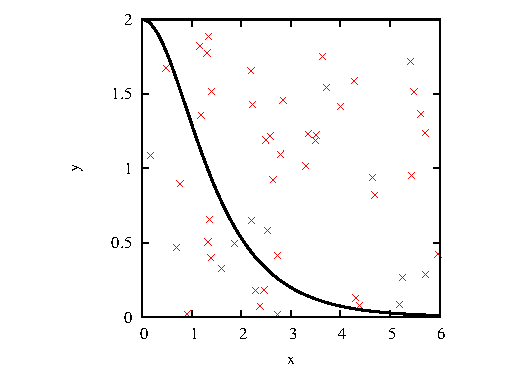
\includegraphics{image/coth-1.pdf}}
\end{frame}

\begin{frame}[t,fragile]{統計誤差の評価}
  \begin{itemize}
    \setlength{\itemsep}{1em}
  \item このモンテカルロ積分が実際に評価している積分
    \[
    \frac{1}{2c} \int_0^c \!\! \int_0^2 \!\! \theta(x,y) \, dx \, dy
    \ \ \ \theta(x,y) = \begin{cases} 2c & \text{if $y < f(x)$} \\ 0 & \text{otherwise} \end{cases}
    \]
  \item 統計誤差の評価
    \begin{itemize}
      \item 試行の成功確率(success probability): $q=\frac{\pi}{2c}$
      \item 一回の試行の平均値(mean): $\mu = 2c \times q = \pi$
      \item 分散(variance):
        \[ s^2 = (2c)^2q + 0^2(1-q) - \mu^2 = 2c\pi-\pi^2 = 4c^2 q(1-q) \]
      \item $c=20$ の時:
        \[ q \simeq 0.0785 \ \ \ s^2 \simeq 116
        \]
    \end{itemize}
  \end{itemize}
\end{frame}

\begin{frame}[t,fragile]{中心極限定理(central limiting theorem)}
  \begin{itemize}
    %\setlength{\itemsep}{1em}
  \item $M$回の試行のうち $N$回成功する確率 ($\pi$の見積もり値が $m=2cN/M$ となる確率)
    \[
    p(m=2c\frac{N}{M}) = \frac{M!}{N!(M-N)!} q^N (1-q)^{M-N}
    \]
  \item 両辺の対数をとってスターリングの公式を使う
    \[
    \log p(m) \simeq \frac{M}{2c} (m \log \frac{\pi}{m} + (2c-m)\log \frac{2c-\pi}{2c-m})
    \]
  \item $m$ に関して平均値 $\pi$ の周りで二次まで展開
    \[
    \log p(m) \simeq -\frac{M}{2s^2}(m-\pi)^2
    \]
  \item 分散$s^2/M$の正規分布(中心極限定理)
  \item 統計誤差は $\sqrt{M}$ に反比例して減少 $\Rightarrow$ 1桁小さくするには100倍の計算が必要
  \end{itemize}
\end{frame}

\begin{frame}[t,fragile]{単純サンプリング(2)}
  \begin{itemize}
    \setlength{\itemsep}{1em}
  \item $y$ に関してあらかじめ積分
  \item $[0,c]$の一様乱数 $x$ を用いて
    \[
    \int_0^c \frac{f(x)}{p(x)} p(x) \, dx \simeq \frac{1}{M} \sum_i c f(x_i) \ \ \ p(x) = \frac{1}{c}
    \]
    \begin{tabular}{|c|c|c|}
      \hline
      $M$ & 平均値 & 誤差 \\
      \hline
      100 & 3.1 & 0.8 \\
      10000 & 3.00 & 0.08 \\
      1000000 & 3.147 & 0.008 \\
      \hline
    \end{tabular}
  \end{itemize}
  \vspace*{-7em}
  \hspace*{17em}
  \resizebox{!}{.45\textheight}{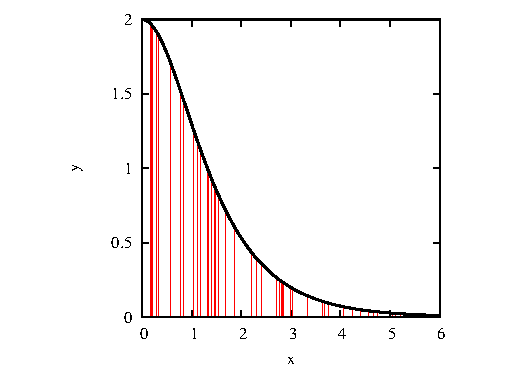
\includegraphics{image/coth-2.pdf}}
\end{frame}

\begin{frame}[t,fragile]{誤差の評価}
  \begin{itemize}
    \setlength{\itemsep}{1em}
  \item 関数 $f(x)/p(x)$ の分散
    \[
    s^2 = \int_0^c \Big(\frac{f(x)}{p(x)}\Big)^2 p(x) \, dx - \pi^2 = c \int_0^\infty f^2(x) \, dx - \pi^2 = 4c - \pi^2
    \]
  \item $c=20$ のとき $s^2 \simeq 70.1$
  \item 同じ試行回数 $M$ の時, 誤差は$\sqrt{70.1/116} = 0.77$ 倍
  \item もしくは $M$ を $116/70.1 = 1.65$ 倍したのと同じ効果
  \item 積分次元は低ければ低いほど良い
  \end{itemize}
\end{frame}

\begin{frame}[t,fragile]{次元の呪い(curse of dimensionality)}
  \begin{itemize}
    %\setlength{\itemsep}{1em}
  \item $n$次元超立方体(1辺の長さ 2, 体積 $2^n$)に対する$n$次元単位球の体積の割合
    \[
    q = \frac{\pi^{n/2} / \Gamma(\frac{n}{2}+1)}{2^n} \sim (\pi/n)^{n/2}
    \]
    $n=10$ で 0.2\%, $n=20$ で $10^{-8}$, $n=100$ で $10^{-70}$
  \item モンテカルロ積分で球の体積を計算しようとすると, 標準偏差に対する平均値の割合は指数関数的に小さい
    \[
    \frac{q}{\sqrt{q(1-q)}} \sim \sqrt{q}
    \]
  \item 次元が高くなるにつれて指数関数的に大きな $M$ が必要となる
  \item c.f. 通常の数値積分(台形公式等)でも同様
  \end{itemize}
\end{frame}

\begin{frame}[t,fragile]{重点的サンプリング}
  \begin{itemize}
    \setlength{\itemsep}{1em}
  \item (平均値が同じなら)被積分関数の分散が小さければ小さいほど良い (= 統計誤差が小さい)
  \item サンプリングの分布 $p(x)$ の形が $f(x)$ に近い程良い
  \item $f(x)$ の値が大きい所はより頻繁にサンプリング
  \item 重点的サンプリング (importance sampling)
  \end{itemize}
\end{frame}

\begin{frame}[t,fragile]{重点的サンプリング}
  \begin{itemize}
    \setlength{\itemsep}{1em}
  \item 積分への寄与が大きな箇所をより重点的にサンプリング
    \[
    p(x) = e^{-x}
    \]
    \begin{tabular}{|c|c|c|}
      \hline
      $M$ & 平均値 & 誤差 \\
      \hline
      100 & 3.06 & 0.06 \\
      10000 & 3.142 & 0.006 \\
      1000000 & 3.1412 & 0.0006 \\
      \hline
    \end{tabular}
  \end{itemize}
  \vspace*{-7em}
  \hspace*{17em}
  \resizebox{!}{.45\textheight}{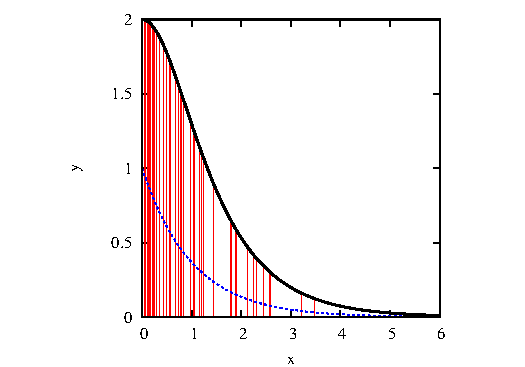
\includegraphics{image/coth-3.pdf}}
\end{frame}

\begin{frame}[t,fragile]{誤差のサンプル数依存性}
  \begin{itemize}
    \setlength{\itemsep}{1em}
  \item 関数 $f(x)/p(x)$ の分散
    \[
    s^2 = \int_0^c \Big(\frac{f(x)}{p(x)}\Big)^2 p(x) \, dx - \pi^2 \simeq 2(2+\pi) - \pi^2 = 0.414
    \]
  \item 同じ試行回数 $M$ の時, 誤差は

    $\sqrt{0.414/116} = 0.06 \mbox{倍}$

  \item もしくは $M$ を 280 倍したのと同じ
  \vspace*{-5em}
  \hspace*{15em}
  \resizebox{!}{.45\textheight}{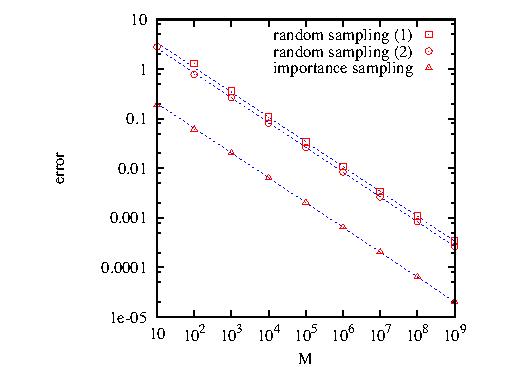
\includegraphics{image/sech-error.pdf}}
  \end{itemize}
\end{frame}

\begin{frame}[t,fragile]{理想的な重点的サンプリング?}
  \begin{itemize}
    \setlength{\itemsep}{1em}
  \item 理想的には $p(x)$ を $f(x)$ に比例するように取れば良い
  \item このとき $f(x) / p(x)$ は定数(分散 0) → 1回のサンプリングで厳密な結果が得られる???
  \item 実際には $p(x)$ が確率密度となるように規格化条件から定数 $c$ を決めておく必要あり
    \[
    \int p(x) \, dx = c \int f(x) \, dx = 1
    \]
  \item $c$ は今欲しい答そのもの!
  \end{itemize}
\end{frame}
